\section{Граничный ранг}

\begin{definition}
  \textbf{Полунепрерывность} функции является более слабым свойством, чем непрерывность. \textbf{Функция полунепрерывна сверху в точке}, если значения функции в близких точках не сильно превышают значение функции в ней. \textbf{Функция полунепрерывна снизу в точке}, если значения функции в близких точках не сильно меньше значения функции в ней.
\end{definition}
Над $\mathbb{R}$ и $\mathbb{C}$ матричный ранг является полунепрерывным. Пусть
\[
	\mathbb{C}^{n \times n} \ni A_j \to A = \lim_{j \to \infty} A_j.
\]
Будем обозначать ранг матрицы $M$ через $rk(M)$. Если для всех $j$ верно $rk(A_j) \leq r$, то $rk(A) \leq r$. Неравенство $rk(A_j) \leq r$ означает, что все $(r+1) \times (r+1)$-миноры обнуляются. (Напомню, что $k \times k$-минором матрицы $A$ называют определитель квадратной матрицы $B$, составленной из элементов матрицы $A$, стоящих на пересечении каких-то $k$ столбцов и каких-то $k$ строк.) Но так как миноры являются непрерывными функциями, то все $(r+1) \times (r+1)$-миноры $A$ также обнуляются.

Тоже самое будет верно для трёхмерных тензоров. Рассмотрим произведение многочленов первой степени от одной переменной по модулю $X^2$:
\[
	(a_0+a_1 X)(b_0 + b_1 X)= a_0 b_0 + (a_1 b_0 + a_0 b_1)X + a_1 b_1 X^2.
\]
Тензор, соответствующий двум билинейным формам $a_0 b_0$ и $a_1 b_0 + a_0 b_1$, имеет ранг 3:
\begin{align*}
  \begin{array}{|c|c|}
  \hline
  1 & 0 \\
  \hline
  0 & 0\\
  \hline
 \end{array}  & \;\;\;\;
 \begin{array}{|c|c|}
  \hline
  0 & 1 \\
  \hline
  1 & 0\\
  \hline
 \end{array} 
\end{align*}

Напомню, что ранги билинейной задачи и её тензора совпадают. В данном случае мы решаем билинейную задачу $F = \left\{ a_0 b_0, a_1 b_0 + a_0 b_1 \right\}$. Чтобы найти её ранг, нужно узнать скольких произведений вида
\[
	P_{\lambda} = \left( \alpha_{\lambda 0} a_0 + \alpha_{\lambda 1} a_1 \right) \cdot \left( \beta_{\lambda 0} b_0 + \beta_{\lambda 1} b_1 \right), 1 \leq \lambda \leq \ell
\]
будет достаточно, чтобы $F$ была в линейной оболочке $lin_{\mathbb{C}}\left\{ P_1, \dotsc, P_{\ell} \right\}$, то есть чему равно число $\ell$.

Чтобы показать, что ранг $F$ больше или равен 3, будем использовать метод подстановок. Сначала положим $a_0=0, b_0=1$. Тогда нам всё ещё нужно вычислить $a_1$, значит есть произведение, зависящее от $a_1$. Скажем, пусть один из его множителей равен $\alpha_{\lambda 0} a_0 + \underbrace{\alpha_{\lambda 1} a_1}_{\neq 0}$. Тогда, заменив $a_1$ на $- \frac{\alpha_{\lambda 0}}{\alpha_{\lambda 1}} a_0$, сможем избавиться от одного произведения. После этого мы будем решать более простую задачу $F' = \left\{ a_0 b_0, -\frac{\alpha_{\lambda 0}}{\alpha_{\lambda 1}}a_0 b_0 + a_0 b_1 \right\}$. Если мы присвоим $a_0=1, b_0=0$, то всё ещё будем вычислять $b_1$. Мы сможем избавиться от другого произведения, выполнив аналогичную подстановку для $b_1$, а именно пусть один из множителей равен $\beta_{\lambda 0} b_0 + \beta_{\lambda 1} b_1$, тогда подставим $-\frac{\beta_{\lambda 0}}{\beta_{\lambda 1}} b_0$ вместо $b_1$.  После всего этого мы всё ещё должны вычислить $F'' = \left\{ a_0 b_0  \right\} $, что требует одного произведения. Очевидно, что ранг будет меньше равен 3, так как 
\[
	F  = \left\{ a_0 b_0, a_1 b_0 + a_0 b_1 \right\} \subseteq lin_{\mathbb{C}}\left\{ P_1 = a_0 b_0, P_2 = a_1 b_0, P_3 = a_0 b_1 \right\}.
\] 

\phantomsection
\label{border_rank_2}
Однако мы можем аппроксимировать тензор, упомянутый выше, с помощью тензоров c рангом два. Пусть
\[
	t(\varepsilon)=(1,\varepsilon) \otimes (1,\varepsilon) \otimes (0, \frac{1}{\varepsilon}) + (1,0) \otimes (1,0) \otimes (1, -\frac{1}{\varepsilon}).
\]

Очевидно, что $t(\varepsilon)$ имеет ранг два для любого $\varepsilon > 0$. Слои $t(\varepsilon)$ будут выглядеть следующим образом
\begin{align*}
  \begin{array}{|c|c|}
  \hline
  1 & 0 \\
  \hline
  0 & 0\\
  \hline
 \end{array}  & \;\;\;\;
 \begin{array}{|c|c|}
  \hline
  0 & 1 \\
  \hline
  1 & \varepsilon\\
  \hline
 \end{array} 
\end{align*}
Поэтому $t(\varepsilon) \to t$, когда $\varepsilon \to 0$.

Бини и др. \cite{Bini} использовали этот эффект, чтобы разработать лучший алгоритм для перемножения матриц. Они начали со следующего частичного матричного умножения:
\[
	\begin{pmatrix}
	  x_{11} & x_{12}\\
	  x_{21} & x_{22} 
	\end{pmatrix}
	\left( 
	\begin{array}{c|c}
	  y_{11} & y_{12}\\
	  y_{21} & \cancel{y_{22}}
	\end{array}
	 \right)
	 =
	 \left( 
	\begin{array}{c|c}
	  z_{11} & z_{12}\\
	  z_{21} & \cancel{z_{22}}
	\end{array}
	 \right),
\]
где они хотели вычислить только три элемента результирующей матрицы. Получаем, что $R(\left\{ z_{11}, z_{12}, z_{21} \right\})=6$, хотя можно приблизительно вычислить $\left\{ z_{11}, z_{12}, z_{21} \right\}$, используя только пять умножений.

То что ранг равен шести, можно показать используя метод подстановок. Рассмотрим $z_{12}$. Ясно, что он зависит от $y_{12}$, поэтому существует произведение, у которого один из множителей равен $y_{12} + \ell(y_{11}, y_{21}, y_{22})$, где $\ell$ --- это линейная форма. Подстановка $y_{12} \to -\ell(y_{11}, y_{21}, y_{22})$ повлияет только на $z_{12}$. После неё мы всё ещё вычисляем $\overline{z_{12}}=x_{11}(-\ell(y_{11},y_{21},y_{22})) + x_{12}y_{22}$. Билинейная форма $\overline{z_{12}}$ всё ещё зависит от $y_{22}$. Поэтому можно снова выполнить подстановку $y_{22} \to -\ell'(y_{11}, y_{21})$. Это уничтожит два произведения, и мы всё ещё вычисляем $z_{11},z_{21}$.

Рассмотрим следующие пять произведений:
\begin{align*}
  p_1 & = (x_{12} + \varepsilon x_{22})   y_{21}\\
  p_2 & = x_{11} (y_{11} + \varepsilon y_{12})\\
  p_3 & = x_{12} (y_{12} + y_{21} + \varepsilon y_{22})\\
  p_4 & = (x_{11} + x_{12} + \varepsilon x_{21}) y_{11}\\
  p_5 & = (x_{12} + \varepsilon x_{21}) (y_{11} + \varepsilon y_{22})
\end{align*}
Получим, что
\begin{align*}
  \varepsilon z_{11}   & = \varepsilon p_1 + \varepsilon p_2 + O(\varepsilon^2)\\
  \varepsilon z_{12} & = p_2 - p_4 + p_5 + O(\varepsilon^2)\\
  \varepsilon z_{21} & = p_1 - p_3 + p_5 + O(\varepsilon^2)
\end{align*}

Теперь возьмём вторую копию того же частичного матричного умножения с новыми переменными. Используя эти две копии, можно перемножать $2 \times 2$ и $2 \times 3$-матрицы (при помощи отождествления некоторых переменных в копии). Поэтому мы можем приблизительно вычислить $\left\langle 2,2,3 \right\rangle$ с помощью 10 умножений. Если бы приближение было бы так же хорошо как точное вычисление, то мы получили бы из этого $\omega \leq 2.79$.

Формализуем концепцию приближения. Пусть $K$ --- поле, и $\widehat{K}:=K[[\varepsilon]]$. (Напомню, что $K[[\varepsilon]]$ обозначает множество всех формальных степенных рядов от переменной $\varepsilon$.) Пусть теперь $\varepsilon$ обозначает неизвестную, а не малую величину как в начале подраздела.

\begin{definition}\label{def:bi:5.1}
	Пусть $h \in \mathbb{N}, t \in K^{k \times m \times n}$.
	\begin{enumerate}
		\item $R_h(t) = \min\{ r \mid \exists u_\rho \in K[\varepsilon]^k, v_\rho \in K[\varepsilon]^m, w_\rho \in K[\varepsilon]^n : \sum_{\rho=1}^r u_{\rho} \otimes v_{\rho} \otimes w_{\rho} = \varepsilon^h t + O(\varepsilon^{h+1}) \}$
		\item $\underline{R}(t)=\min\limits_h R_h(t)$, $\underline{R}(t)$ называется \textbf{граничным рангом} $t$.
	\end{enumerate}
\end{definition}

\begin{remark}\label{rem:bi:5.2}\ 
	\begin{enumerate}
		\item $R_0(t)= R(t)$
		\item $R_0(t) \geq R_1(t) \geq \dotsb = \underline{R}(t)$
		\item Для $R_h$ в $u_{\rho}, v_{\rho}, w_{\rho}$ достаточно будет рассматривать степени вплоть до $\varepsilon^h$.
	\end{enumerate}
\end{remark}

\begin{theorem}\label{th:bi:5.3}
  Пусть $t \in K^{k \times m \times n}, t' \in K^{k' \times m' \times n'}$. Мы имеем
  \begin{enumerate}
       \item $\forall \pi \in S_3: R_h(\pi t) = R_h(t)$.\label{itm:1:th:bi:5.3}
       \item $R_{\max \left\{ h, h' \right\}}(t \oplus t') \leq R_h(t) + R_{h'}(t')$.\label{itm:2:th:bi:5.3}
       \item $R_{h+h'}(t \otimes t') \leq R_{h}(t) \cdot R_{h'}(t')$.\label{itm:3:th:bi:5.3}
  \end{enumerate} 
\end{theorem}
\begin{proof}\ 
  \begin{enumerate}
       \item Очевидно.
       \item Без ограничения общности положим $h \geq h'$. Существуют приблизительные вычисления такие, что
       \begin{align*}
         \sum_{\rho=1}^r u_{\rho} \otimes v_{\rho}  \otimes w_{\rho} & = \varepsilon^h t + O(\varepsilon^{h+1}) \\
         \sum_{\rho=1}^{r'} \varepsilon^{h-h'} u_{\rho}' \otimes v_{\rho}'  \otimes w_{\rho}' & = \varepsilon^{h-h'}\left( \varepsilon^{h'} t' + O(\varepsilon^{h' + 1}) \right) = \varepsilon^h t' + O(\varepsilon^{h+1})
       \end{align*}
       Теперь можно объединить два эти вычисления, так же как делали раньше в случае рангов.
       \item Пусть $t=(t_{ij \ell})$ и $t'=(t_{i' j' \ell'}')$. Имеем $t \otimes t' = (t_{i j \ell} \cdot t_{i' j' \ell'}') \in K^{k k' \times m m' \times n n'}$. Возьмём два приблизительных вычисления для $t$ и $t'$, наподобие тех, что были выше. Если смотреть на них, как на точные вычисления в поле $K[[\varepsilon]]$, то их тензорное произведение вычисляется следующим образом:
       \begin{align*}
         T = \varepsilon^h t + \varepsilon^{h+1} \widehat{t}, &\;\;\;  T' = \varepsilon^{h'} t' + \varepsilon^{h' + 1} \widehat{t}',
       \end{align*}
       где $\widehat{t} \in K[\varepsilon]^{k \times m \times n}$ и $\widehat{t}' \in K[\varepsilon]^{k' \times m' \times n'}$. Их тензорное произведение будет вычислять:
       \begin{align*}
         T \otimes T' & = (\varepsilon^h t_{ij \ell} + \varepsilon^{h+1} \widehat{t}_{ij \ell})(\varepsilon^{h'} t_{i'j'\ell'}' + \varepsilon^{h' + 1}\widehat{t}_{i'j'\ell'}')\\
         & = (\varepsilon^{h+h'}t_{ij \ell} t_{i'j'\ell'}' + O(\varepsilon^{h+h'+1}))\\
         & = \varepsilon^{h+h'} t \otimes t' + O(\varepsilon^{h + h' + 1})
       \end{align*}
       Но это будет приблизительным вычислением для $t \otimes t'$. \qedhere
  \end{enumerate}
\end{proof}

Следующая лемма покажет, что можно превращать приблизительные вычисления в точные.
\begin{lemma}\label{lem:bi:5.4}
  Существует константа $c_h$ такая, что для всех $t$: $R(t) \leq c_h R_h(t)$. $c_h$ зависит полиномиально от $h$, в частности $c_h \leq \binom{h+2}{2}$.
\end{lemma}
\begin{remark}
  \textit{(Наилучшая оценка для $c_h$)} Над конечными полями даже $c_h=1 + 2h$ будет достаточно.
\end{remark}
\begin{proof}
  Пусть $t$ будет тензором с граничным рангом $r$ и пусть
  \[
  	\sum_{\rho=1}^r \underbrace{\left( \sum_{\alpha=0}^h \varepsilon^\alpha u_{\rho \alpha} \right)}_{\in K[\varepsilon]^k} \otimes \left( \sum_{\beta=0}^h \varepsilon^\beta v_{\rho \beta} \right) \otimes \left( \sum_{\gamma=0}^h \varepsilon^\gamma w_{\rho \gamma} \right) = \varepsilon^h t + O(\varepsilon^{h+1}).
  \]
  \begin{figure}[H]
	\centering
    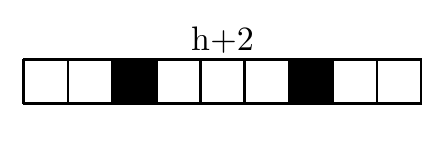
\includegraphics[width=0.3\textwidth]{figures/decomposition}
	\caption{Выбрав два из $h+2$ квадратов, получим разложение $h$ на три части. Поэтому существует всего $\binom{h+2}{2}$ таких разложений.}
	\label{fig:bi:5.1}
  \end{figure}
  Левую часть уравнения можно переписать следующим образом:
  \[
  	\sum_{\rho=1}^r \sum_{\alpha=0}^h \sum_{\beta=0}^h \sum_{\gamma=0}^h \varepsilon^{\alpha+\beta+\gamma} u_{\rho \alpha} \otimes v_{\rho \beta} \otimes w_{\rho \gamma}.
  \]
  Сравнивая коэффициенты при степенях $\varepsilon$, увидим, что $t$ является суммой всех $u_{\rho \alpha} \otimes v_{\rho \beta} \otimes w_{\rho \gamma}$, где $\alpha + \beta + \gamma = h$. Поэтому всё, что необходимо, это вычислить $\binom{h+2}{2}$ произведений.
\end{proof}

В качестве первой попытки использования полученных результатов сделаем следующее:
\begin{align*}
  R_1(\left\langle 2,2,3 \right\rangle)   & \leq 10 \\
  R_1(\left\langle 3,2,2 \right\rangle)   & \leq 10 & (\text{Теорема } \ref{th:bi:5.3}.\ref{itm:1:th:bi:5.3})\\
  R_1(\left\langle 2,3,2 \right\rangle)   & \leq 10 \\
  R_3(\left\langle 12,12,12 \right\rangle)& \leq 1000 & (\text{Теорема } \ref{th:bi:5.3}.\ref{itm:3:th:bi:5.3})\\
  \implies R(\left\langle 12,12,12 \right\rangle) & \leq \binom{3+2}{2} \cdot 1000 = 10 \cdot 1000 = 10000
\end{align*}
Но легко можно получить, что $R(\left\langle 12,12,12 \right\rangle) \leq 12^3 = 1728$. Оказывается, что лучше сначала возвести в тензорную степень, а затем превратить приближённое вычисление в точное.
\begin{theorem}\label{th:bi:5.6} 
  Если $\underline{R}(\left\langle k,m,n \right\rangle) \leq r$, то $\omega \leq 3 \log_{kmn} r$.
\end{theorem}
\begin{proof}
  Пусть $M=kmn$ и пусть $R_h(\left\langle k,m,n \right\rangle) \leq r$. По теореме \ref{th:bi:5.3} получим, что $R_{3h}(\left\langle M,M,M \right\rangle) \leq r^3$ и $R_{3hs}(\left\langle M^s, M^s, M^s \right\rangle) \leq r^{3s}$ для всех $s$. По лемме \ref{lem:bi:5.4} это даст $R(\left\langle M^s, M^s, M^s \right\rangle) \leq c_{3hs} r^{3s}$. Поэтому
  \begin{align*}
    \omega  & \leq  \log_{M^s} (c_{3hs} r^{3s})\\
    & = 3s \log_{M^s}(r) + \log_{M^s}(c_{3hs})\\
    & = 3 \log_M(r) + \underbrace{\frac{1}{s} \log_M(\text{ многочлен от } s)}_{\to 0 \text{ при } s \to \infty}.
  \end{align*}
  Так как $\omega$ является инфимумом, то получим $\omega \leq 3 \log_M(r)$.
\end{proof}

\begin{corollary}
  $\omega \leq 2.79 \dotso$
\end{corollary}
